\documentclass{article}
\usepackage[utf8]{inputenc}
\usepackage[spanish]{babel}
\selectlanguage{spanish}
\usepackage{graphicx}
\usepackage{float}

\title{Facultad de Ciencias \\Tarea-Examen 1 \\ Fundamentos de Bases de Datos}
\author{Arteaga Hérnandez Alejandro Iabin \and Barocio Gómez Luis Fernando}

\date{Fecha de entrega: 13 Marzo 2020}

\begin{document}

\maketitle
Instrucciones: Lee cuidadosamente los enunciados del examen antes de comenzar a resolverlos. Deberás justificar todas las respuestas. El examen deberá entregarse en clase el miércoles 13 de marzo de 2020. El examen se puede entregar en parejas. 
\begin{enumerate}
    %%%%%%Pregunta 1%%%%%%%%%
    \item (15 puntos) Contesta las siguientes preguntas:
    \begin{itemize}
        \item Describe brevemente los tres niveles de la arquitectura ANSI SPARK: externo, conceptual y físico
        \begin{itemize}
            \item Externo: Una vista de usuario describe una parte de la base de datos que es relevante para un usuario en particular. Excluye datos irrelevantes, así como los datos que el usuario no está autorizado a acceder.
            
            \item Conceptual: El nivel conceptual es una forma de describir los datos que se almacenan dentro de la base de datos y cómo los datos están relacionados entre sí. Este nivel no especifica cómo se almacenan físicamente los datos.   
            
            \item Físico: El nivel interno implica la forma en que la base de datos se representa físicamente en el sistema informático. En él se describe cómo los datos se almacenan en la base de datos y en el hardware del equipo.
        \end{itemize}
        
        
        \item ¿Qué ventajas y desventajas encuentras al trabajar con una base de datos?
        
        Ventajas:
        \begin{itemize}
            \item Proveen facilidades para la manipulación de grandes volúmenes de datos.
            
            \item Simplifican la programación de equipos de consistencia.
            
            \item Organizan los datos con un impacto mínimo en el código de los programas.
            
            \item Usualmente, proveen interfaces y lenguajes de consulta que simplifican la recuperación de los datos.
        \end{itemize}
        
        Desventajas:
        \begin{itemize}
            \item Si se tienen muy pocos datos que son usados por un único usuario por vez y no hay que realizar consultas complejas sobre los datos, entonces es posible que sea mejor usar una planilla de cálculo.
            
            \item Coste de la BD, los requisitos de hardware para correr una base de datos por lo general son relativamente altos, por lo que estos equipos pueden llegar a costar gran cantidad de dinero.
            
            \item En caso de un accidente que corrompa la Base de datos, el proceso de recuperación  y de devolver a  la Base de Datos su estado anterior al problema, es mucho mas complejo de ejecutar que en sistemas tradicionales. 
            
        \end{itemize}
        
        \item ¿Qué es la independencia de datos? ¿Qué es la independencia lógica? ¿Qué es la independencia física? ¿Cuál es más difícil de lograr?
        \begin{itemize}
            \item ¿Qué es la independencia de datos? La independencia de datos se puede definir como la capacidad para modificar el esquema en un nivel del sistema sin tener que modificar el esquema del nivel inmediato superior.
            
            \item ¿Qué es la independencia lógica? Es la capacidad de modificar el esquema conceptual sin tener que alterar los esquemas externos ni los programas de aplicación. Se puede modificar el esquema conceptual para ampliar la base de datos o para reducirla.
            
            \item ¿Qué es la independencia física? es la capacidad de modificar el esquema interno sin tener que alterar el esquema conceptual (o los externos).
            
            \item ¿Cuál es más difícil de lograr? Dado que la independencia física solo se refiere  a la separación entre las aplicaciones y las estructuras físicas de almacenamiento, es más fácil de conseguir que la independencia lógica.
            
        \end{itemize}
        
        
        \item Realiza un diagrama para describir cada una de las fases que involucran el ciclo de vida de una Base de Datos. 
            \begin{figure}[htbp]
            \centering
            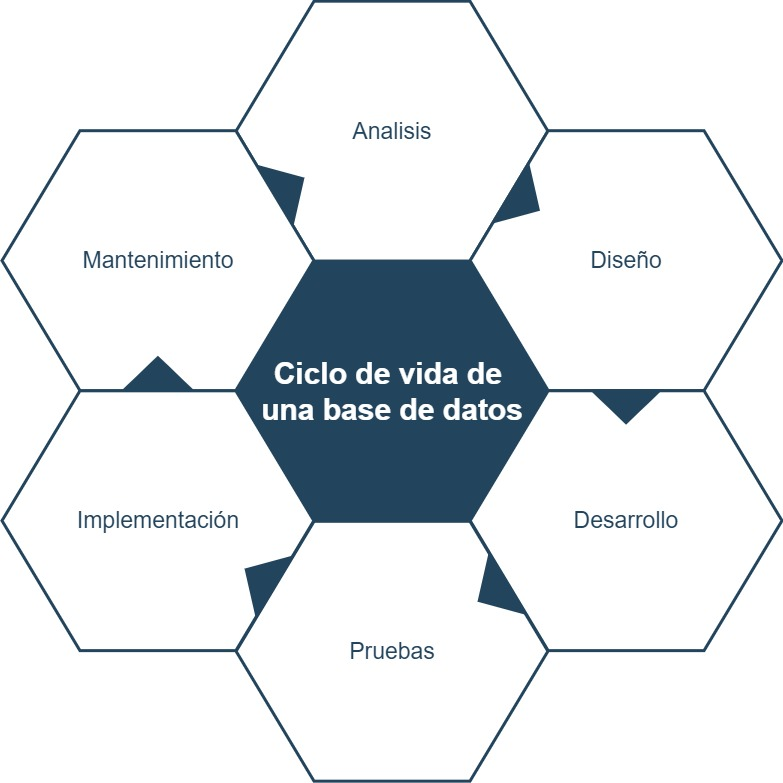
\includegraphics[scale=0.16]{CicloBD.jpg}
            \end{figure}
        
        \item ¿Qué es un tipo de entidad y qué una instancia de entidad?
        Una entidad es un objeto exclusivo único en el mundo real que se está controlando y una instancia de entidad es contenido concreto de la base de datos en un momento dado. Varía con el tiempo, al añadir, eliminar o modificar datos, utilizando el lenguaje de modificación de datos 
        
        \item ¿Qué es un tipo de relación y una instancia de relación? 
        Los tipos de relaciones son asociaciones entre tablas que se crean utilizando sentencias de unión para recuperar datos y la instancia de relación son objetos que hay dentro del modelo de datos de instancia de relación que tienen atributos que contienen los datos que deberán utilizarse para una relación de búsqueda.
        
        \item Indica cómo se maneja el concepto de agregación en el modelo E/R y proporciona un ejemplo ilustrativo. ¿Cuáles son los beneficios (o no) de dicho concepto? Agregación en E/R es “descomponer” la entidad en entidades más pequeñas y con ello podemos usarla en caso de necesitar ser más específicos a la hora de relacionar y trata a la entidad como de un nivel superior.
        \begin{figure}[htbp]
            \centering
            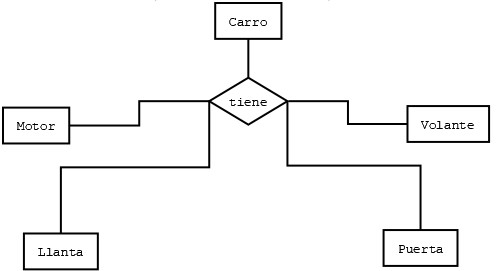
\includegraphics[scale=0.6]{1ER.jpg}
            \end{figure}

        
        \item Indica cuáles son las restricciones que se pueden definir en el modelo E/R, así como sus características más importantes.
        \begin{itemize}
            \item Cardinalidad. Cantidad de entidades que pueden participar en la relación.
            \begin{itemize}
                \item Uno a uno: Una entidad en A se asocia sólo con una entidad en B, y una entidad en B se asocia sólo con una entidad en A
                
                \item Uno a varios: Una entidad en A se asocia con cualquier número de entidades en B, pero una entidad en B se puede asociar sólo con una entidad en A.

                \item Varios a uno: Una entidad en A se asocia sólo con una entidad en B, pero una entidad en B se puede asociar con cualquier número de entidades en A.
                
                \item Varios a varios: Una entidad en A se asocia con cualquier número de entidades en B, y una entidad en B se asocia con cualquier número de entidades en A.
                
                \end{itemize}
            
            \item Participación. Determina la obligatoriedad de participación de una entidad en una relación. Sus características son:
            \begin{itemize}
                \item Parcial
                
                \item Total o dependencia de existencia
                
                \item Débil
            \end{itemize}

        \end{itemize}
        
        \item Utiliza un par de ejemplos (en cada caso) de la vida real para ilustrar las restricciones de cardinalidad y participación, disponibles en el modelo E/R.
        
        \begin{itemize}
            \item Uno a uno.
                \begin{figure}[ht]
                \centering
                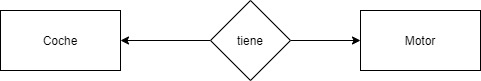
\includegraphics[scale=0.3]{Preguntaunoejemplos1.jpg}
                \end{figure}
            
            \item Uno a varios.
                \begin{figure}[ht]
                \centering
                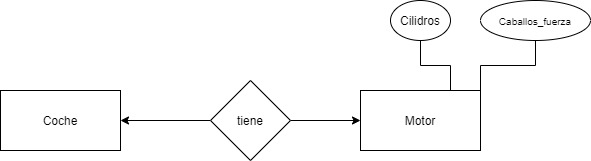
\includegraphics[scale=0.3]{Preguntaunoejemplos2.jpg}
                \end{figure}
            
            \item Varios a uno. 
                \begin{figure}[ht]
                \centering
                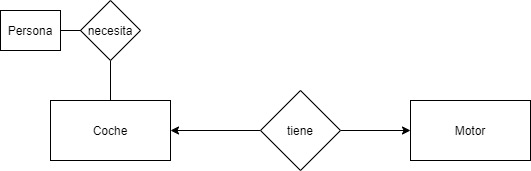
\includegraphics[scale=0.3]{Preguntaunoejemplos3.jpg}
                \end{figure}
            
            \item Varios a varios.
                \begin{figure}[hbt!]
                \centering
                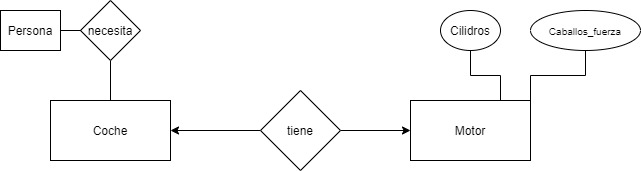
\includegraphics[scale=0.3]{Preguntaunoejemplos4.jpg}
                \end{figure}
            
            \item Parcial
                \begin{figure}[hbt!]
                \centering
                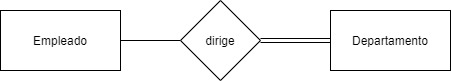
\includegraphics[scale=0.3]{Preguntaunoejemplos5.jpg}
                \end{figure}
            
            \item Total
                \begin{figure}[hbt!]
                \centering
                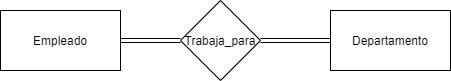
\includegraphics[scale=0.3]{Preguntaunoejemplos6.jpg}
                \end{figure}
            
        \end{itemize}
        
    \end{itemize}
    %%%%%%Pregunta 2%%%%%%%%%
    \item (15 puntos) Estrella de la Muerte  
        Hace mucho tiempo, en una Galaxia muy, muy lejana, el malvado Imperio Galáctico comenzó la construcción de su última arma, la Estrella de la Muerte, una estación espacial blindada con suficiente poder para destruir un planeta entero. Este terror tecnológico almacenará toda su información en una base de datos relacional, y se te ha pedido diseñar un esquema E/R. La solicitud que ha hecho el Emperador es la siguiente: 
        
        \begin{itemize}
            \item La Estrella de la Muerte emplea una fuerza de trabajo de más de 200,000 trabajadores. Cada trabajador tiene asignado un número de identificación Imperial, un nombre y rango. Los trabajadores pueden ser oficiales, soldados de asalto, pilotos, artilleros o personal de apoyo de la estación. Todo el personal de la estación tiene un oficial al mando
            
            \item La estación se divide en varios niveles, cada uno identificado por un número. La base de datos debe realizar un seguimiento de la superficie total de un nivel, la capacidad de almacenamiento, y si se trata de un nivel restringido o no. Todos los niveles tienen viviendas con capacidad alojar a varios trabajadores, y a todos los trabajadores se les asignan viviendas en la estación. 
            
            \item Algunos de los niveles de la estación pueden tener bloques de celdas para prisioneros y estos bloques de celdas se identifican por una sola letra que es única dentro de un nivel; sin embargo, estas letras se pueden repetir entre los niveles. Cada celda tiene una cierta capacidad de prisioneros (no es la misma para todas). Para los bloques de celdas se debe llevar un registro de la fecha de entrada y la fecha de ejecución del prisionero. Los prisioneros tienen un identificador único, un nombre y una afiliación (por ejemplo, la escoria Rebelde). 

            \item Algunos de los niveles de la estación funcionan como hangares, donde se tienen cruceros imperiales, naves de reconocimiento y de ataque. Cada nave tiene un identificador único, capacidad de vuelo, personal asignado (oficiales, pilotos, personal de apoyo, soldados, etc.), armamento y hangar al que está asignada. 
        \end{itemize}    
    Dibuja un diagrama Entidad/Relación que represente la información antes mencionada. Indica las llaves subrayando los atributos, restricciones de cardinalidad y de participación. 
    
    \begin{figure}[htbp]
            \centering
            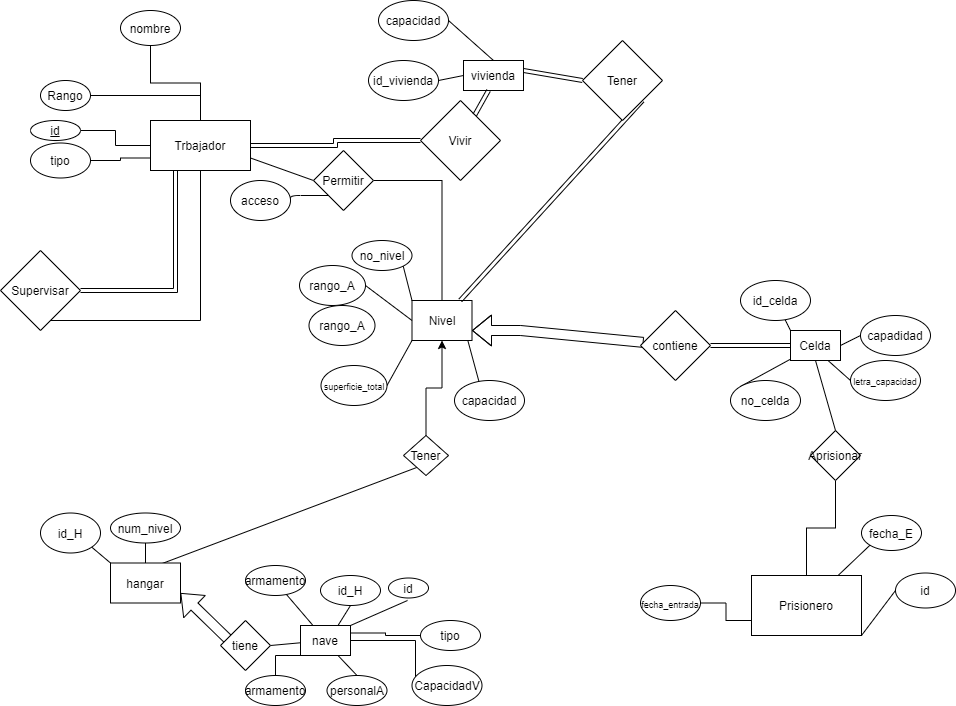
\includegraphics[scale=0.5]{Estrella .png}
    \end{figure}
    \newpage
    
    %%%%%%Pregunta 3%%%%%%%%%
    \item (10 puntos) Ingeniería inversa:
    
    \begin{itemize}
        \item PaqueteTV (clavePaquete, tipoPaquete, precio, equiposAdicionales)
        \item Persona (CURP, nombre, paterno, materno, dirección, estado)
        \item Contratar (CURP, clavePaquete) 
        
        \begin{itemize}
            \item ¿Indica qué modela el esquema anterior? Dibuja un diagrama Entidad/Relación equivalente: ¿cuáles deberían ser los identificadores?, indica las restricciones (cardinalidad y participación) que debiera tener. 
            \par\null\par
            El identificador de la entidad \textbf{paqueteTv} es \textbf{clavePaquete} debido a que esta es única por cada paquete\par\null\par
            De la misma manera el identificador de la entidad \textbf{persona} es \textbf{curp} ya que este es único por cada persona
            \par\null\par
            La relación resultante es una relación \textbf{Muchos a muchos} ya que un paquete puede tener varias personas que lo hayan contratado, y por el otro lado, una persona podría contratar muchos paquetes
            \par\null\oar 
            La participación es parcial para ambas entidades, ya que puede haber paquetes que no hayan sido contratados por nadie y personas que no contraten nada.\par\null\par
            \begin{figure}[ht]
            \centering
            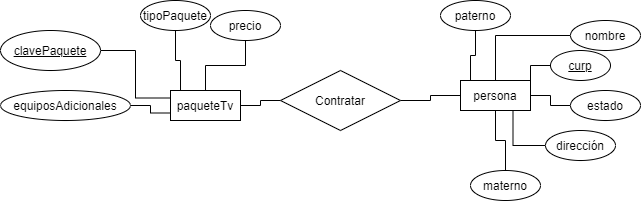
\includegraphics[scale=0.65]{tres (1).png}
            \end{figure}
    
            

            \item  ¿Qué cambios deberías hacer al esquema anterior, si a la empresa le interesara tener información de los instaladores del servicio (se te pide que agregues algunos descriptores para los instaladores), considerando que un instalador también podría contratar el servicio que la empresa oferta
            
            \par\null\par
            Se agrega la entidad \textbf{instalador} y la relación \textbf{ser}, la cardinalidad de la relación es \textbf{uno a uno} ya que una persona solo puede ser un instalador, y un instalador solo puede ser una persona.
            \par\null\par
            Respecto a la cardinalidad, la cardinalidad de la entidad instalador es \textbf{total} debido a que \textbf{todo instalador tiene que ser una persona}
            mientras que la participación de persona es parcial ya que \textbf{no todas las personas son instaladores}
            \par\null\par
            \begin{figure}[ht]
            \centering
            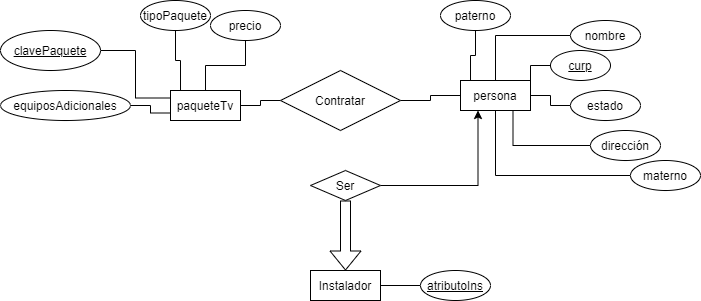
\includegraphics[scale=0.65]{32.png}
            \end{figure}
        \end{itemize}
    \end{itemize}

    %%%%%%Pregunta 4%%%%%%%%%
    \item (15 puntos) Dibuja un diagrama E/R equivalente para el siguiente diseño. Justifica tu respuesta:
    \newpage
        \begin{figure}[ht]
        \centering
        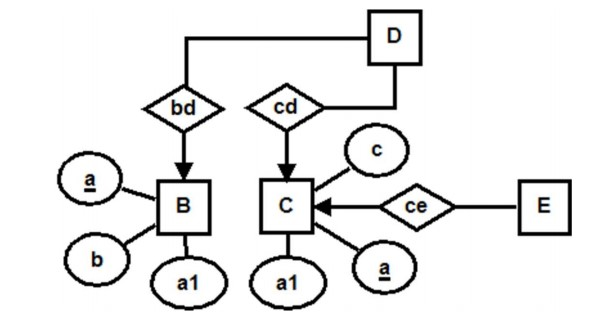
\includegraphics[scale=0.5]{Problema 4.jpg}
        \end{figure}
        \par\null\par
        Debido a que la entidad D, solo tiene puede estar a lo más relacionada con una entidad B, podemos pasar los atributos de la entidad B a la entidad D, de esta manera, cuando no haya relación, estos atributos estarán en NULL, y cuando haya una relación, se pondrán directamente como atributos de D.
        \par\null\par
        Lo mismo se hace para la entidad C, como cada D puede tener un C relacionado, podemos agregar los atributos de C también a la entidad D. y debemos conservar la relación ce, ahora con D porque D tiene los atributos de C.
        \par\null\par
        D conserva su llave primaria que en este caso no tiene, pero si tuviera no cambiaría. 
        \par\null\par
        Los modelos son equivalentes, aunque el segundo es mucho más sucio debido a que habrá mucha redundancia cuando se pase a tablas. 
        \par\null\par
        \begin{figure}[ht]
        \centering
        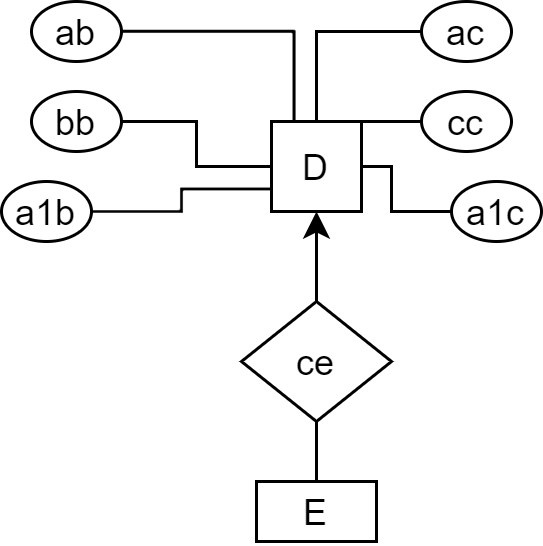
\includegraphics[scale=0.3]{cuatro.png}
        \end{figure}
        
    %%%%%%Pregunta 5%%%%%%%%%
    \item  (10 puntos) Considera las relaciones abc y cd entre las entidades A, B, C y D. No se ha definido ningún tipo de restricción, cómo expresarías (utilizando restricciones), las siguientes reglas de negocio: 
    \begin{enumerate}
        \begin{figure}[h]
        \centering
        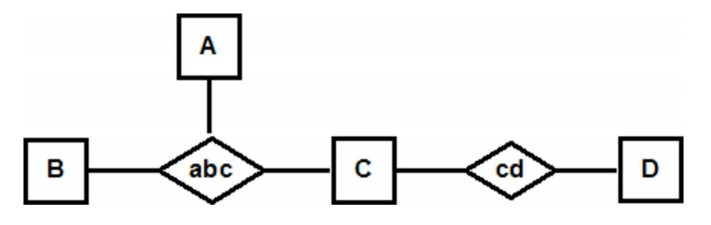
\includegraphics[scale=0.4]{Problema 5.jpg}
        \end{figure}
        
        \item Una ocurrencia de la entidad C sólo puede relacionarse con una ocurrencia de la entidad A. 
         \begin{figure}[h]
        \centering
        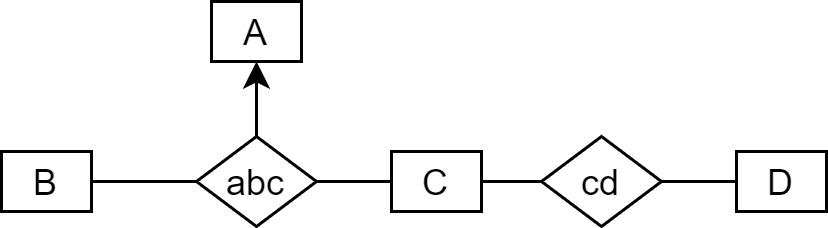
\includegraphics[scale=0.3]{5a.jpg}
        \end{figure}
        \par\null\par
        Pero una A sigue pudiendo relacionarse con muchas C
        \item Las ocurrencias de la entidad B, están obligadas a relacionarse con las de las entidades A o B. 
         \begin{figure}[h]
        \centering
        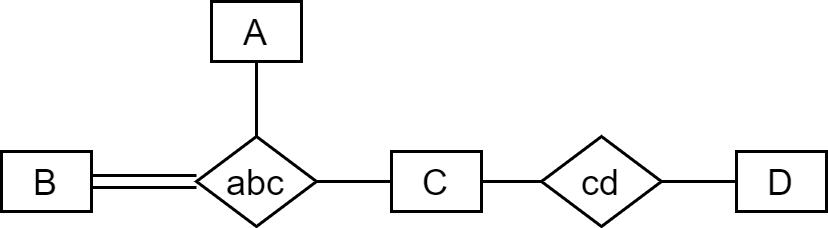
\includegraphics[scale=0.3]{5b.png}
        \end{figure}
        \item Una ocurrencia de la entidad D sólo puede relacionarse con varias ocurrencias de la entidad C
        \par\null\par
        El diagrama original ya cumple esta restricción D ya puede relacionarse con varias ocurrencias de C o con ninguna, pero el enunciado no dice \textbf{debe}.
        \item Una misma ocurrencia de la entidad C puede relacionarse con diferentes ocurrencias de la entidad D al mismo tiempo. 
        \par\null\par
        Eso ya sucede, debido a que la relación cd es \textbf{muchos a muchos} c puede relacionarse con varias entidades D
    \end{enumerate}
    
    
    %%%%%%Pregunta 6%%%%%%%%%
    \item (10 puntos) Indica si el siguiente diagrama Entidad/Relación permite modelar la siguiente situación: Una persona gusta de beber bebidas y las personas beben en un bar en una fecha determinada. Justifica tu respuesta y en caso que no se verifique el escenario planteado, especifica un modelo que si cumpla. 
    
    \begin{figure}[ht]
        \centering
        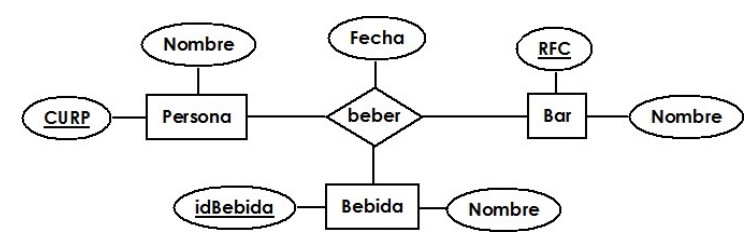
\includegraphics[scale=0.5]{Problema 6.jpg}
        \end{figure}
    
    \par\null\par
    El diagrama E/R mostrado, no tiene una relación para almacenar que gustan beber las personas. Por eso el enunciado.
    \textbf{\textit{Una persona gusta de beber bebidas}} no está modelado en el diagrama.
    \par\null\par
    El segundo enunciado \textbf{\textit{Las personas beben en un bar en una fecha determinada}} Si se puede modelar con el diagrama dado, ya que la relación beber está definida con los atributos mencionados en el enunciado \textbf{Persona,beber,fecha,Bar}
     \par\null\par
     El diagrama propuesto es el siguiente
    \begin{figure}[ht]
        \centering
        
\includegraphics[scale=0.6]{6.png}
        \end{figure}\newpage
    %%%%%%Pregunta 7%%%%%%%%%
    \item (15 puntos) Considera el modelo Entidad/Relación que se propone a continuación, el cual representa la operación de una cadena de farmacias. Responde a las siguientes cuestiones con respecto al modelo presentado: 
    
    \begin{figure}[ht]
        \centering
        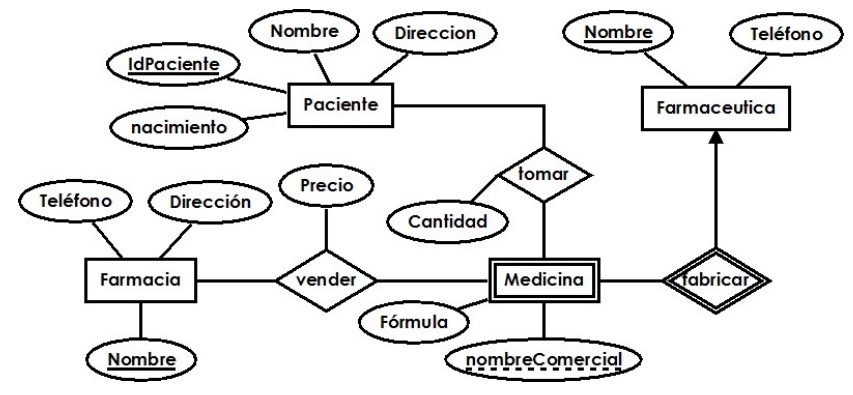
\includegraphics[scale=0.5]{Problema 7.jpg}
        \end{figure}

\begin{enumerate}
    \item ¿Puede una compañía farmacéutica tener múltiples números de teléfono? Si no, ¿qué necesitas hacer para permitir
    esto? 
    \par\null\par
    NO, para permitir eso, podríamos agregar un atributo multivaluado \textbf{teléfono} de esa manera teléfono tendría varios valores, pero cuando pasemos a relacional eso traerá problemas ya que viola la 1FN ya que los atributos no son atómicos, otra opción y la que yo recomendaría, sería agregar una nueva entidad teléfono, y una relación con farmacéutica que sea tener.
    \item Si borráramos de la base de datos a la compañía farmacéutica que fabrica un medicamento, ¿qué sucede con los
    medicamentos que fabrica? Justifica tu respuesta.
    \par\null\par
    Depende de como se configure en el SMDBD, hay varias configuraciones posibles:\\
    ON DELETE RESTRICT Si hay alguna llave foránea haciendo referencia a farmaceutica, el manejador no te dejará.\\
    ON DELETE NO ACTION : lo mismo que restrict\\
    ON DELETE CASCADE : Esta opción, hace que se borren todas las filas en otras tablas que tengan referencia a la fila que borraste, en este caso se borrarán las medicinas de esa farmacéutica.\\
    ON DELETE SET NULL Simplemente pone null en la llave foránea de medicina.
    \item Si en lugar de eliminar la compañía farmacéutica, ¿qué ocurriría si elimináramos la farmacia que vende el
    medicamento? ¿Tendríamos que eliminar el medicamento también? ¿Por qué sí o por qué no?\par\null\par
    \textbf{No}, debido a que como es una relación \textbf{muchos a muchos} la relación vender se pasa como una nueva tabla a la BD, de tal manera que si se borra una farmacia, tendría que hacerse algo con el registro de vender, pero no afectaría en nada a la tabla medicina. Para la tabla vender estarían las opciones que mostré arriba.
    \item ¿Se permite que una farmacia venda medicamentos en exclusiva? En caso que no, ¿qué se necesitaría para permitir
    esta característica? 
    \par\null\par
    \textbf{No} una medicina puede ser vendida por muchas farmacias, si quisiéramos que todas las medicinas fueran vendidas sólo por una farmacia, tendríamos que cambiar la cardinalidad de la relación vender a \textbf{uno a muchos}, pero todas las medicinas solo podrían ser vendidas por una farmacia, si queremos que haya medicinas exclusivas y medicinas normales, tendríamos que crear otra entidad que sería, medicina exclusiva y esa tener una relación vender \textbf{uno a muchos} con farmacia.

\end{enumerate}
    

    %%%%%%Pregunta 8%%%%%%%%%
    \item  (15 puntos) Modifica el modelo mostrado en la pregunta 7 para que pueda representar lo siguiente: 
    \begin{enumerate}
        \item Cada paciente debe tener un único médico de atención primaria. Cada médico tiene al menos un paciente y queremos conocer la cédula, nombre y especialidad. 
         \begin{figure}[ht]
        \centering
        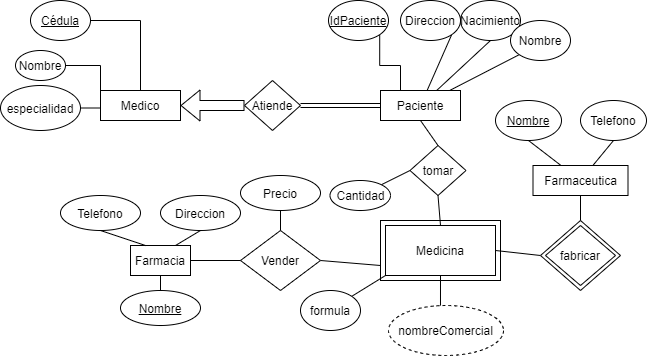
\includegraphics[scale=0.5]{8a.png}
        \end{figure}

        \item El diseño solo modela el hecho de que un paciente toma algunos medicamentos, queremos que ahora el modelo permita que un paciente tome ciertos medicamentos recetados por un médico y la fecha de prescripción. 
       \begin{figure}[ht]
        \centering
        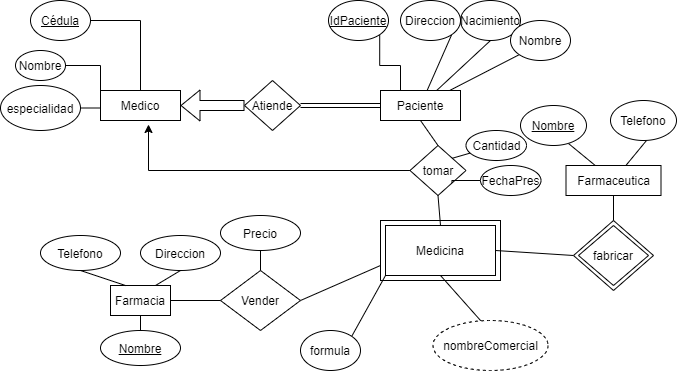
\includegraphics[scale=0.5]{8b.png}
        \end{figure}
\newpage
        \item Las compañías farmacéuticas tienen contratos a largo plazo con farmacias. Un compañía farmacéutica establecer contratos con varias farmacias, y una farmacia puede contratar varias compañías farmacéuticas. Para cada contrato, queremos almacenar la fecha de inicio y la fecha de finalización. 
          \begin{figure}[ht]
        \centering
        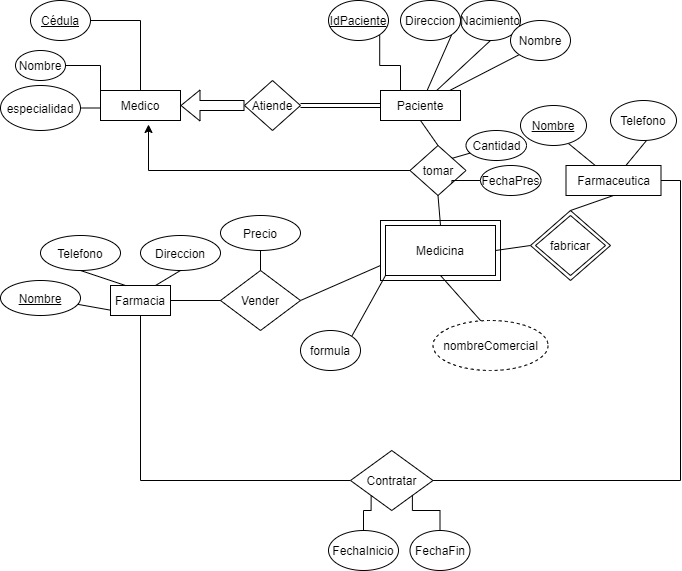
\includegraphics[scale=0.5]{8c.png}
        \end{figure}
    \end{enumerate}
    
\end{enumerate}

\end{document}
